% Boris Vian - Raphaël Lizé

\documentclass[twoside]{book}
\usepackage{hyperref}


\usepackage{graphicx}
\usepackage{subfig}
\usepackage{placeins}


% Unicode encoding  
\usepackage[utf8x]{inputenc}


% Colorfull Text
\usepackage{xcolor}


% \euro
\usepackage{eurosym}


% Language settings:
\usepackage[francais]{babel}

\usepackage[T1]{fontenc}


% Tables
\usepackage{array}
\usepackage{longtable}


% Hyperrefferences  
\usepackage{hyperref}


% Font settings:
\usepackage{kpfonts}


\title{Boris Vian}
\author{Raphaël Lizé}
% Page layout settings
\usepackage{geometry}
\geometry{
	a4paper,  % 21 x 29,7 cm
%	body={160mm,240mm},
%	left=30mm, 
%	top=25mm,
%	headheight=7mm, 
%	headsep=4mm,
%	marginparsep=4mm,
%	marginparwidth=27mm
}


% Spacing:
\usepackage{setspace}


% Headers and footers:
\usepackage{fancyhdr}
\pagestyle{fancy}
          \fancyhf{}
          \fancyfoot[LE,RO]{\textcolor[gray]{0.3}{\thepage}}
          % Rulers width
          \renewcommand{\footrulewidth}{.3pt}
          \renewcommand{\headrulewidth}{.3pt}
\fancyfoot[LO,RE]{\textcolor[gray]{0.3}{Raphaël Lizé}}
\fancyfoot[CO,CE]{\textcolor[gray]{0.3}{Boris Vian}}


% Vars & functs
% Paths
\newcommand\PIXPATH{./docs/pics}
\newcommand\SRCPATH{./docs/src}

% Object:
\newcommand\Object{}

% End of line(forced):
\newcommand\el{\hfill\\}

% Lists design:
\renewcommand{\labelitemi}{$\diamond$}
\renewcommand{\labelenumii}{\arabic{enumi}.\arabic{enumii}}


% Begining of the document
\begin{document}

	%Including all the files:

    % Fichier ./docs/tex/0.premiere_page.tex

% Front Page 
\thispagestyle{empty}

% Title:
\maketitle

% Picture
\begin{center}
    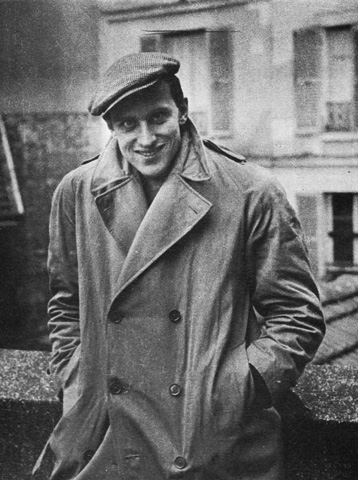
\includegraphics[height=3cm]{\PIXPATH/frontPage}
\end{center}

\vfill
\pagebreak

% Table of contents 
\tableofcontents
\vfill
\pagebreak

    % Fichier ./docs/tex/1.partie1.tex

% Partie 1: présentation du personnage

\section{Boris Vian, Bison Ravi, et tout leurs amis}

% Intro

Il est difficile de parler de Boris Vian. Peut-être parce qu'il
est difficile de lui coller une seule étiquette. Un seul nom,
même. «Boris Vian» pour l'état civil, «Bison Ravi» -- anagramme
de «Boris Vian» pour les proches, «Vernom Sullivan» pour certains
livres, et des dizaines d'autres pseudonymes en tant que chroniqueur.
% TODO: lien liste des pseudonymes (annexes ?)
Mais pour évoquer le personnage, on peut déjà s'intéresser à l'Histoire,
et à son histoire.
% TODO: Annexe frise chrono ?

\subsection{Contexte historique}
Il est nécessaire de décrire le contexte historique de la vie
de Boris Viqn pour comprendre certaines forces externes qui
ont pu avoir une influence significative sur sa vie, ainsi que
sur son oeuvre.

Boris Vian est né peu après la seconde guère mondiale. En 1929, c'est
la crise avec le crash de Wall Street. En 1940, l'Allemagne envahit la
partie nord de la France. Toute une partie de la culture est alors
interdite et censurée, notament le jazz, d'origine noire-américaine.

\subsection{Famille et éducation}

Boris Vian est issu d'une famille riche. Son père, Paul Vian, est rentier
depuis ses 20 ans. Sa mère est l'héritière d'une riche famille de l'industrie
du papier.

Les Vian habitent une grande maison, «Les Fauvettes», à Ville d'Avray, dans la
banlieue de Paris, près du parc de Saint-Cloud. Le plus important est le loisir,
le divertissement, tout ce qui est agréable. Les enfants Vian vivent ainsi coupés
du monde extérieur: la politique, la religion, ou tout autre sujet sérieux n'entre
pas dans ce petit monde clos. On profite de la vie.

Cette maison n'est pas le seul paradis des Vian. Tous les étés, ils se rendent
à Landemer, dans le Cotentin, où les enfants peuvent jouer tout l'été sur la
plage privée de la propriété apportée par la Mme. Vian. 

\subsection{Vie publique, vie privée}


    % Fichier ./docs/tex/2.partie2.tex

% Partie 2: présentation de l'oeuvre

\section{Une oeuvre hétéroclite et en qvqnce sur son temps}

\subsection{}

\subsection{}

\subsection{}

    % Fichier ./docs/tex/3.partie3.tex

% Partie 3: l'héritage

\section{Un héritage riche et une influence encore vive aujourd'hui}

En ayant à l'esprit toutes (ou ne serait-ce même qu'une partie) des activités,
tous les métiers qu'il a éxercé, il aurait été bien étonnant que Boris Vian ne
laisse pas une trace, ne soit pas une source d'influences pour les générations
futures.
C'est effectivement le cas. Son héritage est riche et multiple, et je vais
dévelloper ici les trois principaux aspects (il faut bien choisir) qui me semblent
les plus marquants de ces onfluences.

\subsection{Culture et social}

Boris Vian a laissé sa marque dans le paysage culturel et social français. Déjà
de son vivant, il marquait les esprits, étant un personnage un peu hors-norme; et
certains de ces traits, en plus de ses oeuvres, sont passés à la postérité.

\paragraph{La légende de Saint-Germain-des-Prés}

Qui n'a jamais entendu parler de Saint-Germain-des-Prés ? Je parle bien-sûr
du Saint-Germain de l'après-guerre, le lieu de rencontre des intellectuels et
des artistes parisiens: Sartre, Queneau, Prévert % TODO: citer plus
et bien d'autres. Le soir, la jeuness du tout-Paris se retrouve dans les caves
des établissements du quartier, dansant (et buvant) toute la nuit au son jazz
noir-américain. Swing, zfpok et cuite garantis sur facture !

Le surnom de «Prince de Saint-Germain» donné à Boris Vian atteste de son importance
dans ce petit monde, connaissant tous (et toutes \ldots), animant avec ses amis et
ses frères les soirées endiablées, d'abord au \emph{Tabou}, puis une fois la
frénésie des premières années passées, dans l'ambiance plus feutrée du \emph{Club
Saint-Germain}.

Sa connaissance intime de Saint-Germain et de sa faune pousse un éditeur, au moment
ou Saint-Germain et les bachannales qui s'y déroulent deviennent plus connues du
grand public, de demander au «Prince» un «Guide de Saint-Germain-des-Prés».
L'ouvrage, prévu avec force descriptions farfelues et illustrations des gens et
lieux, ne fut hélas pas publié, l'éditeur ayant fait faillite entre-temps.

C'est également dans ces clubs que Boris Vian acceuille ses idole du jazz que sont
Miles Davis, Duke Ellington (son dieu), et bien d'autres \ldots

\paragraph{Langage}

Amateur de langage et de jeux de mots, expérimentateur du verbe et néologiste
patenté, écrivain et homme public: il n'est pas surprenant que des exprseeions
de son cru nou parviennent.
Le meilleur exemple est sans aucun doute l'utilisation du mot «tube».

C'est lors d'une réunion de travail chez Philips en 1957, alors qu'il y ait
directeur artistique, qu'il propose ce mot pour désigner un succès populaire,
ou une chanson qui est assurée d'avoir du succès, parfois malgré l'ineptie du
texte ou la qualité musicale. Boris proposait ce mot pour remplacer l'alors
usité «saucisson». Devant la supériorité objective du candidat, il n'est pas
surprenant qu'il est été adopté -- difficile d'imaginer un \emph{disc jokey}
annoncer le dernier «saucisson» de l'été ! Par la même occasion, Boris Vian a
fourni une alternative viable au \emph{hit} anglais. Cocorico.

\paragraph{La génération 68}

La première large reconnaissance littérarire de Boris Vian -- des oeuvres signées
de son vrai nom s'entend -- fût apportée par la jeunesse de la fin des années 60.
Se sentant représentés par cet auteur si anticonformiste, anticonventionel, dont
le destin tragique à gonflé le myhte de rêveur à le jeunesse éternelle, Boris Vian
et son oeuvre -- en particulier \emph{L'écume de jours} -- ont influencé toute une
génération. En avance sur son temps comme souvent -- même lorsqu'il s'agit de
mourrir ! , Boris Vian n'a malheureusement pas connu cette gloire méritée.

\subsection{Musique}

\subsection{Théâtre}



% The end
\end{document}

